%----------------------------------------------------------------
%
%  File    :  text-only-browsers.tex
%
%  Author  :  Olli-Pekka Riikola, TU Graz, Austria
% 
%  Created :  2.12.2022
% 
%----------------------------------------------------------------


\chapter{Text-Only Browsers}

\section[History of Text Browsers]{A Quick Look to the History of Text-Only Browsers}
\label{tb-history}
Originally, text browsers were the only way to browse the web. Also, back in the days, internet connetion speeds used to be much slower than today but similarly web sites were much simpler and it was possible to access them with even with the narrow bandwidth. After that there is now several powerful graphical web browsers for web users, but the text browsers still have some important usecases even they are quite old solution for web browsing. \parencite{best-text-browsers}. In addition, there is still a few promising text browser remaining and even receiving recent updates at least annually, and they are worth for have a look.

\section{Text-Only Browsers in use}
\label{tb-known}
The header above might seems to be a bit exaggerating, but it is totally possible and sensible to use text browsers in daily basis. This is, because text browsers are lightweight softwares and still efficient on poor internet connection and they could actually help user to reduce distraction while browsing the web and that is why they could be a good choice for a browser even nowadays. The text browsers are designed to logically organize the content of the website rather than just to be ordinary web browser which gives the access to the site for a user. More than that, persons with no sight or who are partially impaired can more efficiently access website with text browser in combination with screen reader. And when talking about blind persons as a web users it is important to consider, that they obviusly can't see or otherwise access the actual graphical pieces of art, images, videos or other similar mediaformats in the website. \parencite[Chapter 2]{webbie} So, text browsers reduces the content that screen readers cannot read and that way they will make the web browsing more convenient for blind people.

\subsection{Common Problems}
\label{tb-problems}
Event the layout of the site would be simple in text browser, it still is not simple in practice. According \textcite[Chapter 5]{webbie} the reason is presentation. People with sight can have advantage of very versatile navigation link list, but for a blind user it might be a struggle. It becomes a struggle at the point, when text browser try to present navigation bar as a list of links, and screen reader starts to read it - link by link, one by one. Luckily, there is an option to skip this navigation bar and go straight to the content, but only if the element is designed properly in the website. Otherwise text browser does not realize that there is a navigation bar, but it just present it like a list of links and user needs to handle it.

Another issue is empty attributes of element, like ALT attribute in IMAGE element. And of course this problem would quite easily be fixed by the programmer, specially with powerful accessibility checking tools, but sadly it is not always like that. So, since images are not relevant content for a person with no sight, it is very important that the ALT tag will tell, what is going on in that part of the website. Also, if image is for hyperlink, then it should also tell with ALT tag, where it will bring the user. \parencite[Chapter 5]{webbie}.

Perhaps, the most difficult issue in the terms of text browser, is dynamic content. Since most text browsers do not support JavaScript, some functionality is not available for the user in the site. This essentially means, that text browsers are not any more so convenient way to browse the web. But still, like mentioned in \ref*{tb-history}, there is few interesting text browser softwares available in the internet.

\section{Known Text-Only Browsers}
\label{tb-browsers}
\subsection{Lynx}
\label{tb-lynx}
Lynx is quite old text browser and it appears to be probably most well known one. But as it is in the \textcite{lynx} website, Lynx is a command line interface WWW client for Unix systems. Interesting sidenote could aslo be, that back in the years the Lynx has been a solution to build Campus Wide Information Systems. 
\subsection{WebbIE}
\label{tb-webbie}
WebbIE is the one, which is designed to help visually impaired persons to access the web. They are dedicated to work in combination with screenreaders, like JAWS, WindowEyes, Thunder, NVDA and Narrator as mentioned in the \textcite{webbie-main} website. WebbIE runs on Windows, and it seems to be pretty much only choice for Windows users.
\subsection{W3M}
\label{tb-w3m}
W3M is also a very handy text browser and it works as pager too, like 'more' or 'less' as it says in \textcite{w3m} website. It also works as text formatting tool from HTML to plain text.
\subsection{Links}
\label{tb-links}
Another interesting and very nicely working text browser is Links which is school project from the days in 1999. But since then it has been kept up to date and many people are involved in the project and put effort to make Links more diverse. \parencite{links}. It runs on Unix.
\subsection{Others}
\label{tb-others}
There is also few cases worth to mention, perhaps even if they are not in the same class with these ones mentioned above. However, there is a project called Browsh, which is a graphical text browser running on Linux. It supports JavaScript, so all functionality in the site should be accessed but it is still very early stage in the development. But it might be useful on poor internet connection. 

Another ones are more like plugins, but it is good to know, that there is still such. Chrome offers a plugin, which makes website like text site, but it seems to be somehow outdated and poor. More interesting and very well working built-in function is Firefox Reader-View. It just makes the website to be easier to read with removing distracting elements and making the content to be more cleary seen. This function can be activated just by pressing F9 in the Firefox browser and it works in several website.
\begin{figure}[tp]
    \centering
    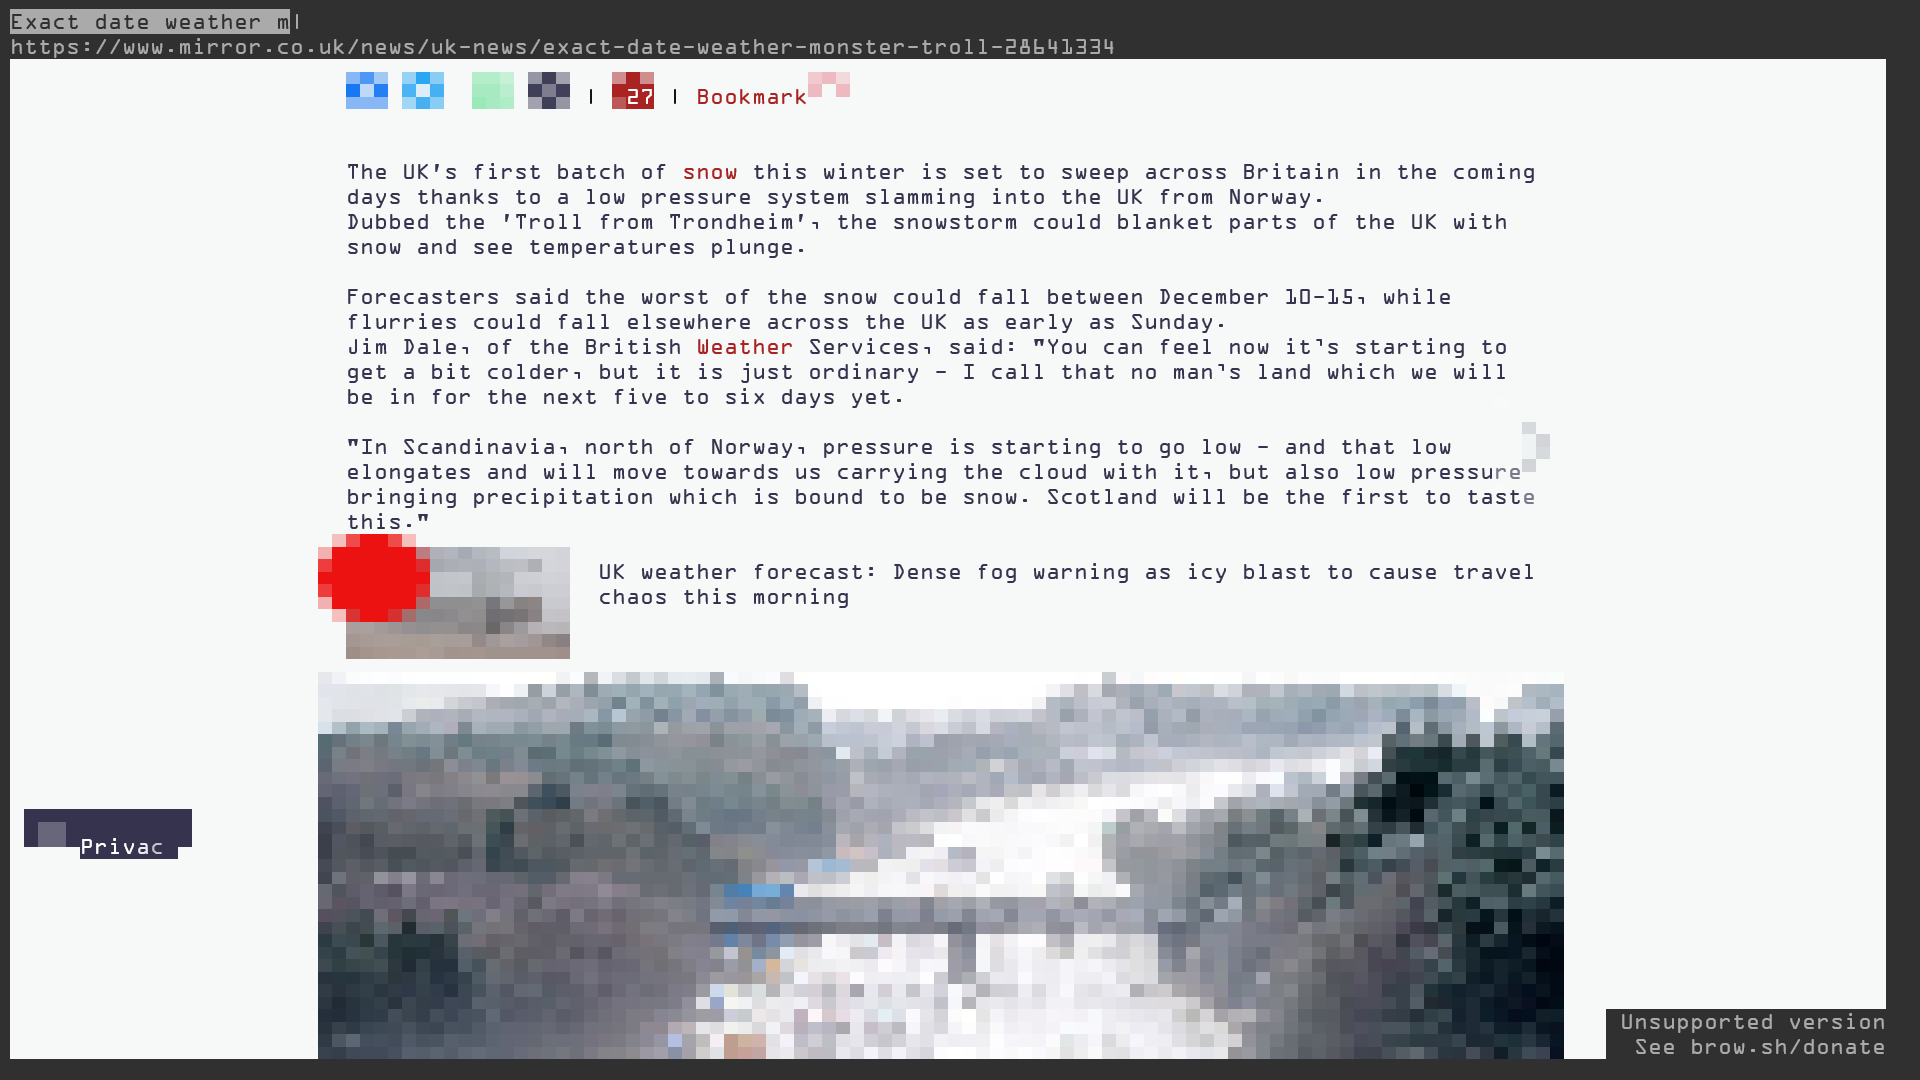
\includegraphics[keepaspectratio,width=\linewidth,height=\halfh]
    {images/browsh.png}
    
    \caption[Browsh grahical CLI browser]
    {%
    Browsing a web with Browsh in website gov.uk.
    }
    \label{fig:browsh}
\end{figure}
\begin{figure}[tp]
    \centering
    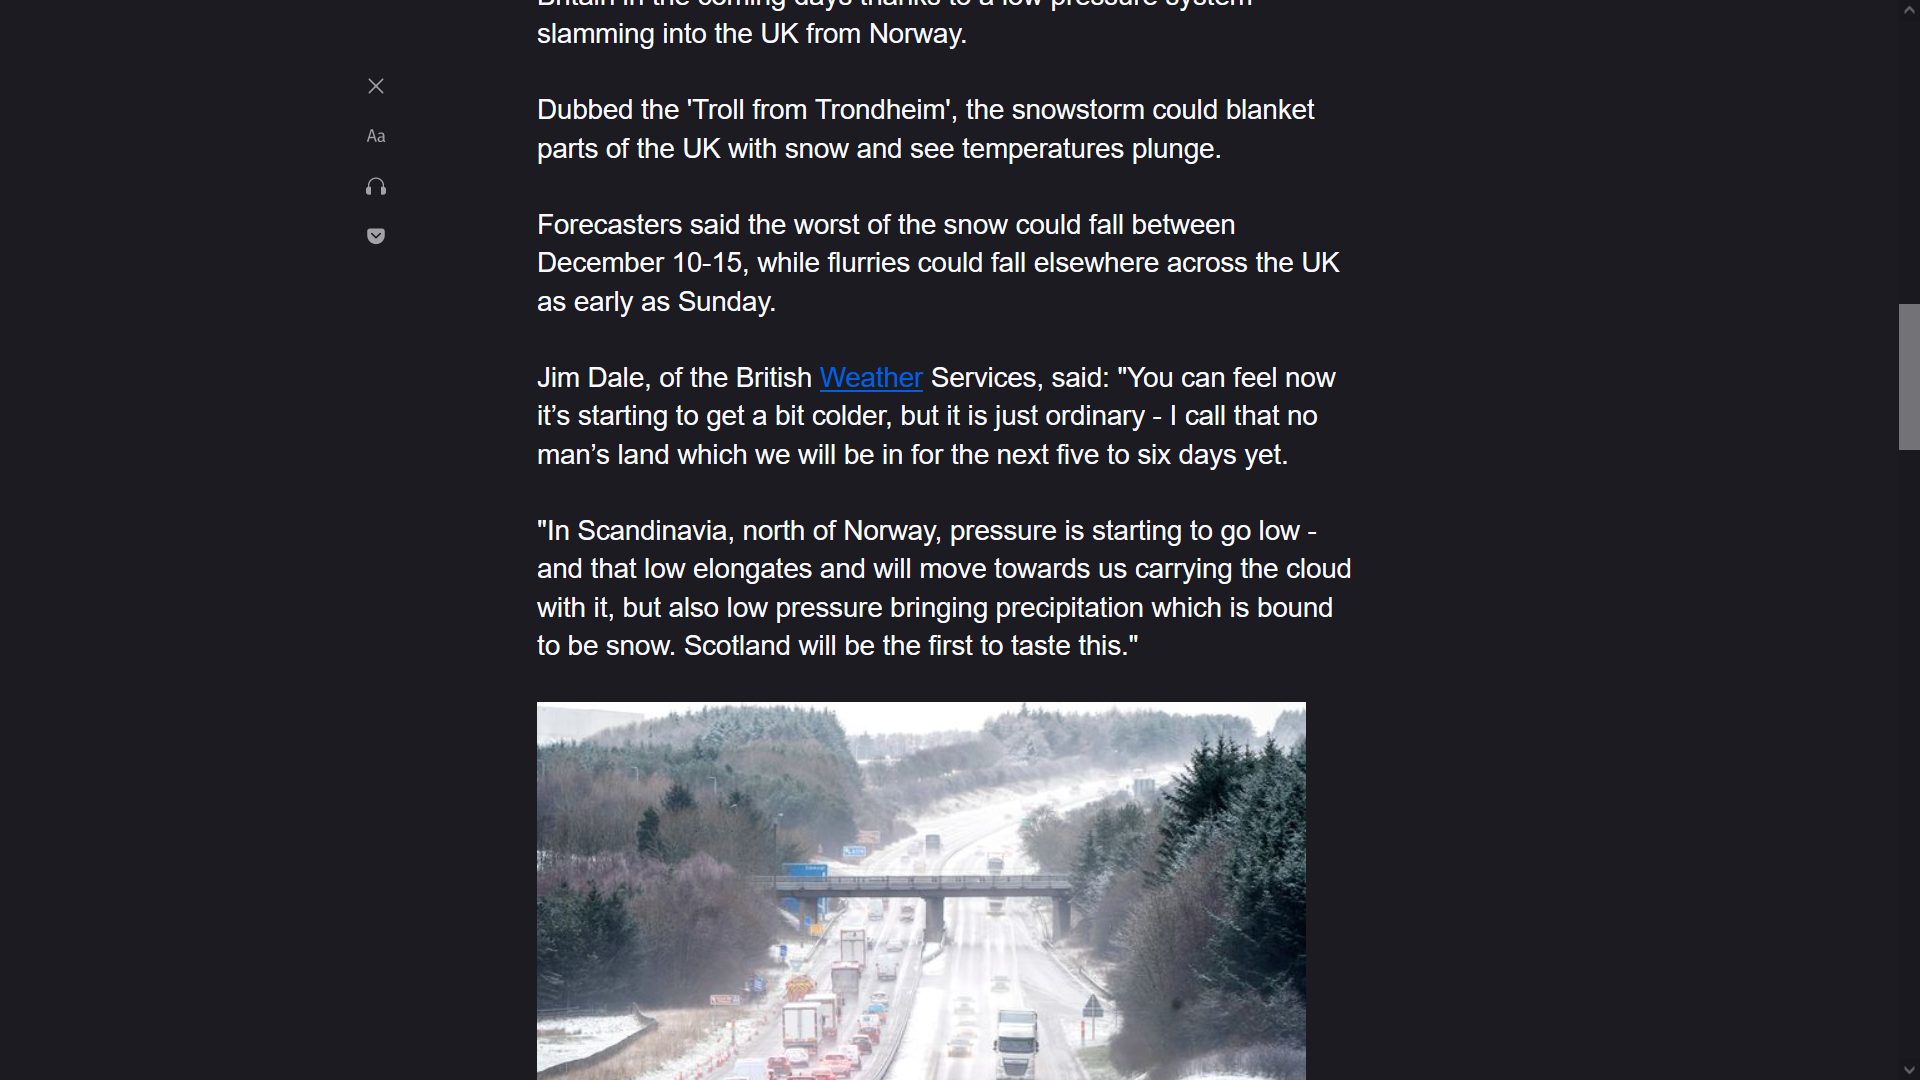
\includegraphics[keepaspectratio,width=\linewidth,height=\halfh]
    {images/reader-view.png}
    
    \caption[Firefox Reader-View]
    {%
    Browsing a web with Firefox Reader-View
    }
    \label{fig:firefox-rv}
\end{figure}
\section{Showcases and Data of Text Browsers}
\label{tb-general}
In this section there is provided practical examples and an interesting data  of these text browsers. Due to siplicity of the text browsers, it is easy to get familiar with them to only watching a showcase video and comparing the screenshots below in the section \ref*{tb-screenshots}.
\subsection{Showcase videos}
\label{tb-showcase}
There is showcase video in YouTube, where is shown what it looks like when browsing the web with the Lynx text browser. In the video it is shown two examples gov.uk and mirror.co.uk, which represents an examples of good and bad web accessibility. Both videos are quite similar in structure, just tabbing through the sites and entering the links, but that way it is easy to recognize the probles with the first glance in the mirror.co.uk website. Link to the showcase video is provided in reference \textcite{tb-showcase}.
\subsection{Screenshots of Text Browsers}
\label{tb-screenshots}
Following images presents how efficient a text browsers actually could be. In the case of mirror.co.uk, even if there is plenty of images and advertisements, the text browsers are able to present the content somehow sensible. In this area, most interesting examples is Lynx and WebbIE. Others are more or less similar than the Lynx - only thing to consider is, that W3M and Links works responsively inside of CLI, Lynx does not. 

\begin{figure}[tp]
    \begin{minipage}{0.48\linewidth}
        \centering
        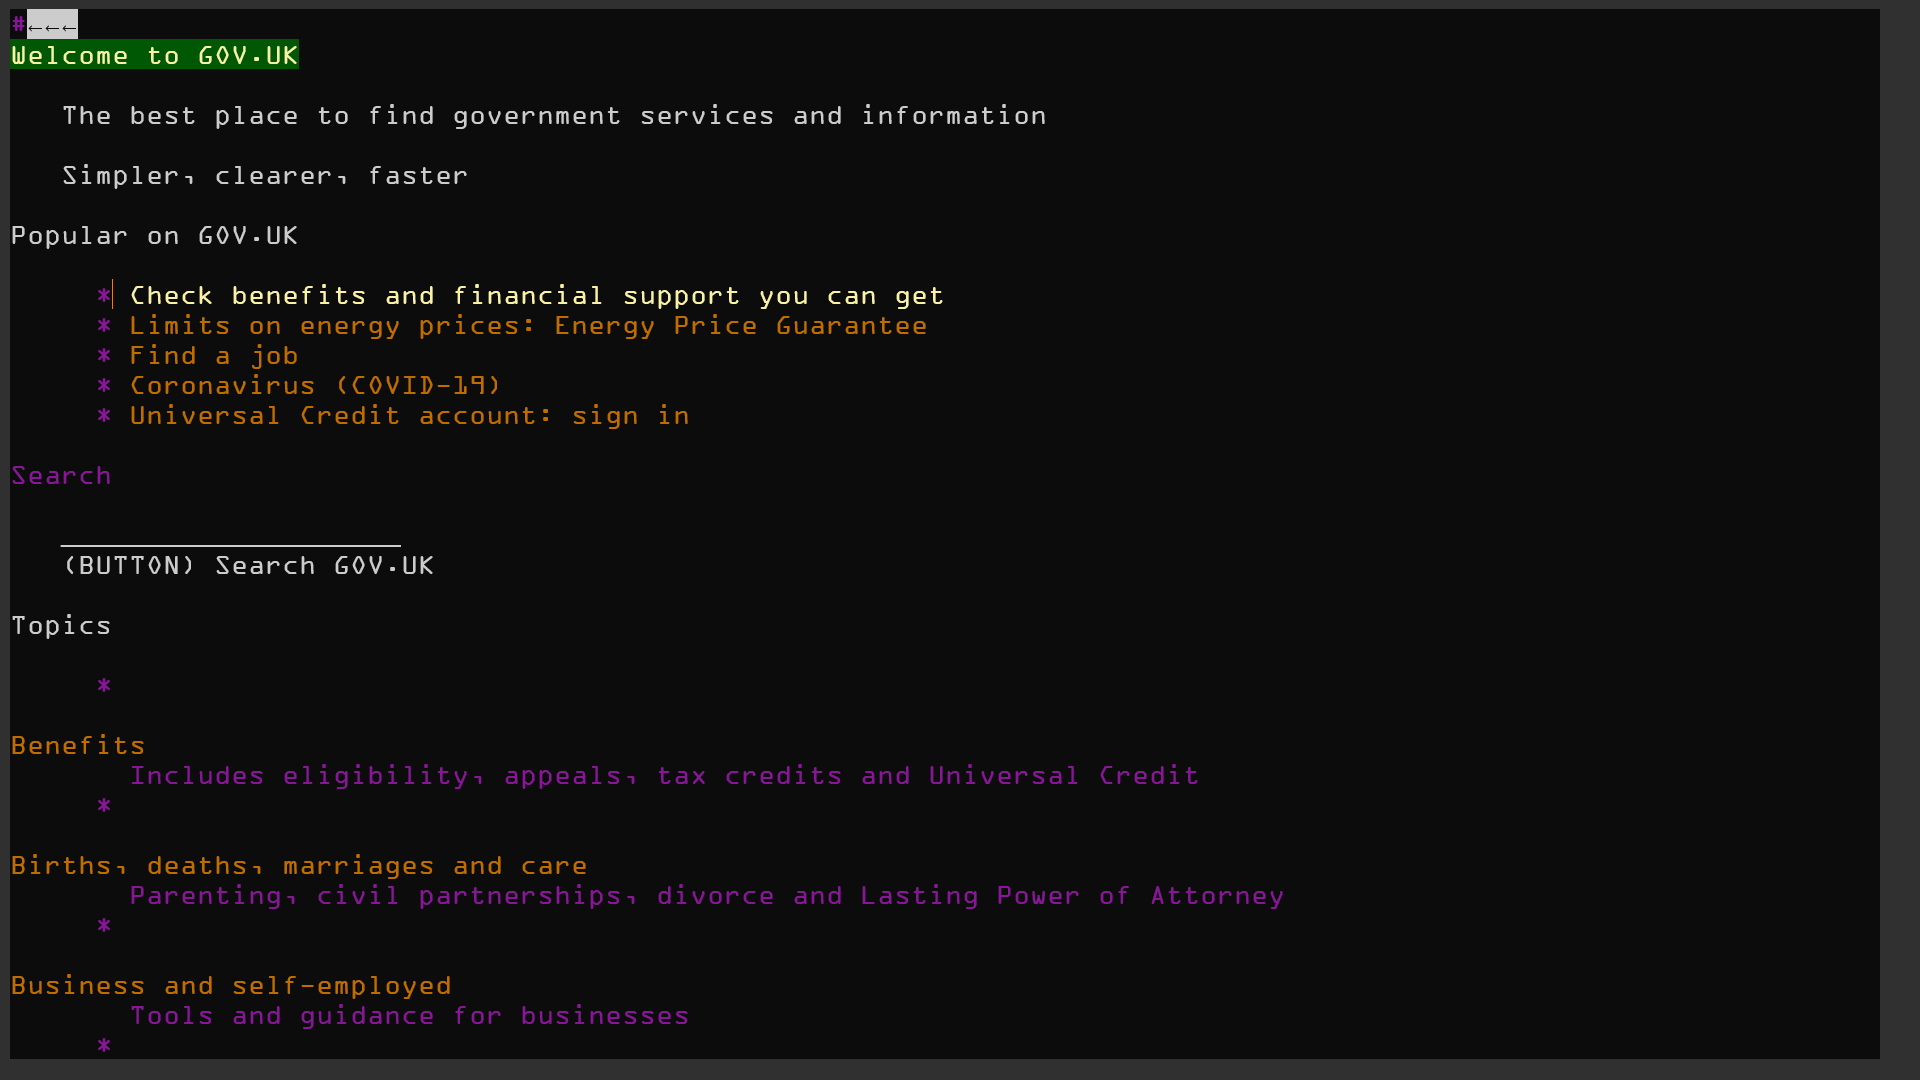
\includegraphics[keepaspectratio,width=\linewidth]
        {images/lynx-gov}
        
        \caption[Lynx browser]
        {%
        Browsing the gov.uk website
        }
        \label{fig:lynx-gov}
    \end{minipage}\hfill
    \begin{minipage}{0.48\linewidth}
        \centering
        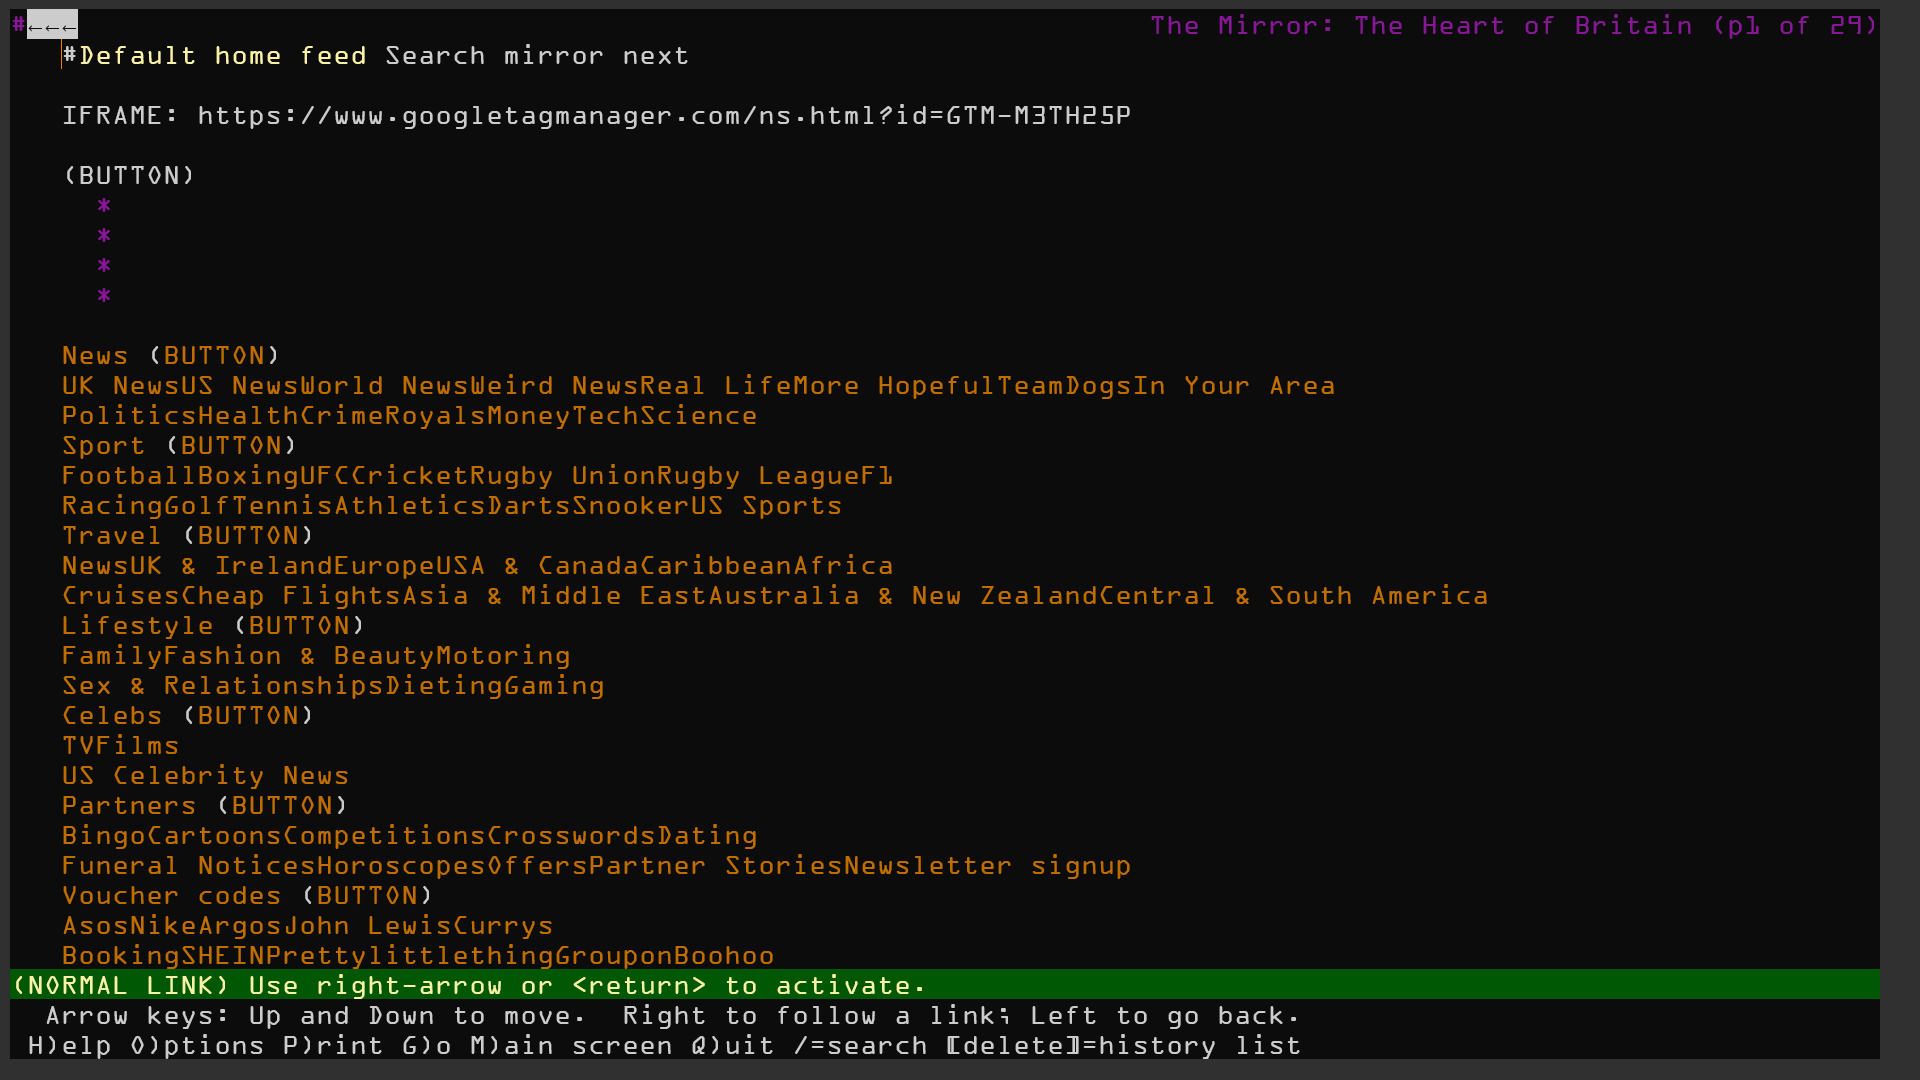
\includegraphics[keepaspectratio,width=\linewidth]
        {images/lynx-mirror}
        
        \caption[Lynx browser]
        {%
        Browsing the mirror.co.uk website
        }
        \label{fig:lynx-mirror}
    \end{minipage}
\end{figure}

\begin{figure}[tp]
    \begin{minipage}{0.48\linewidth}
        \centering
        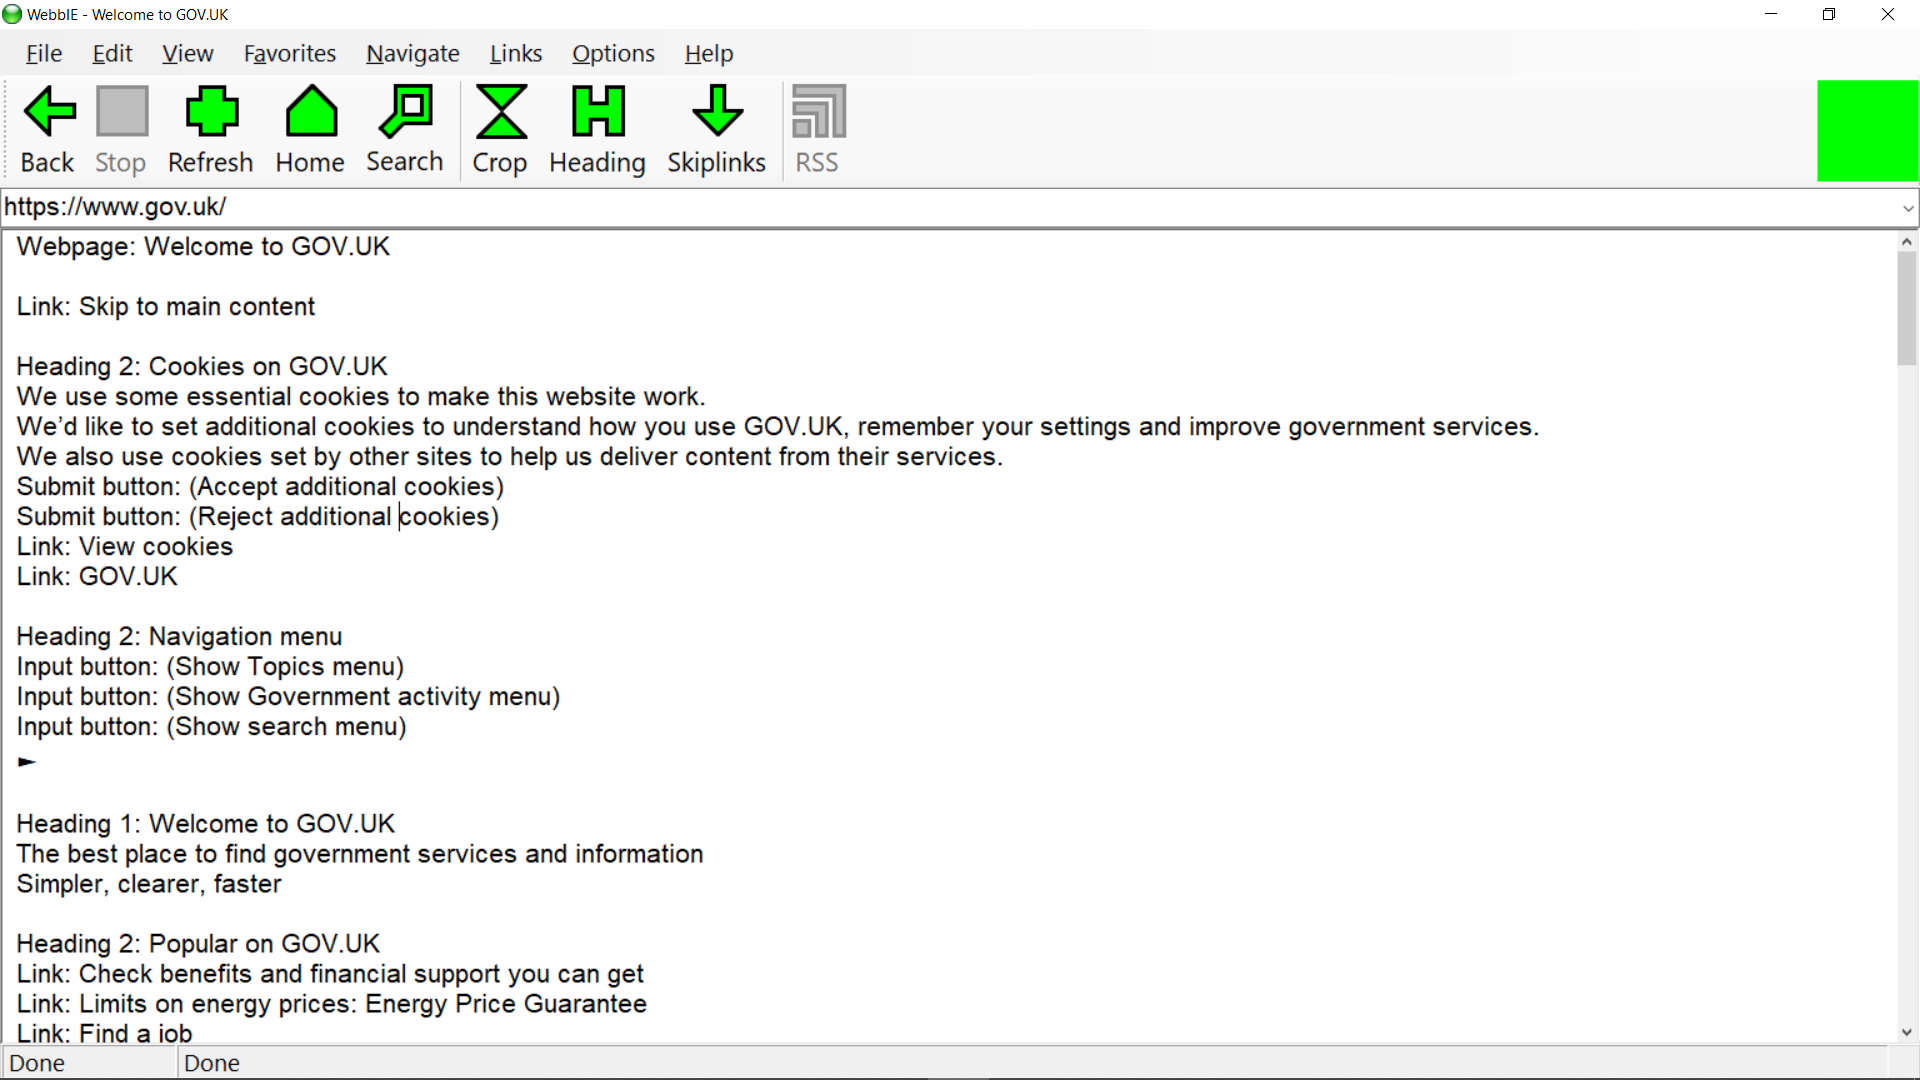
\includegraphics[keepaspectratio,width=\linewidth]
        {images/webbie-gov}
        
        \caption[WebbIE browser]
        {%
        Browsing the gov.uk website
        }
        \label{fig:webbie-gov}
    \end{minipage}\hfill
    \begin{minipage}{0.48\linewidth}
        \centering
        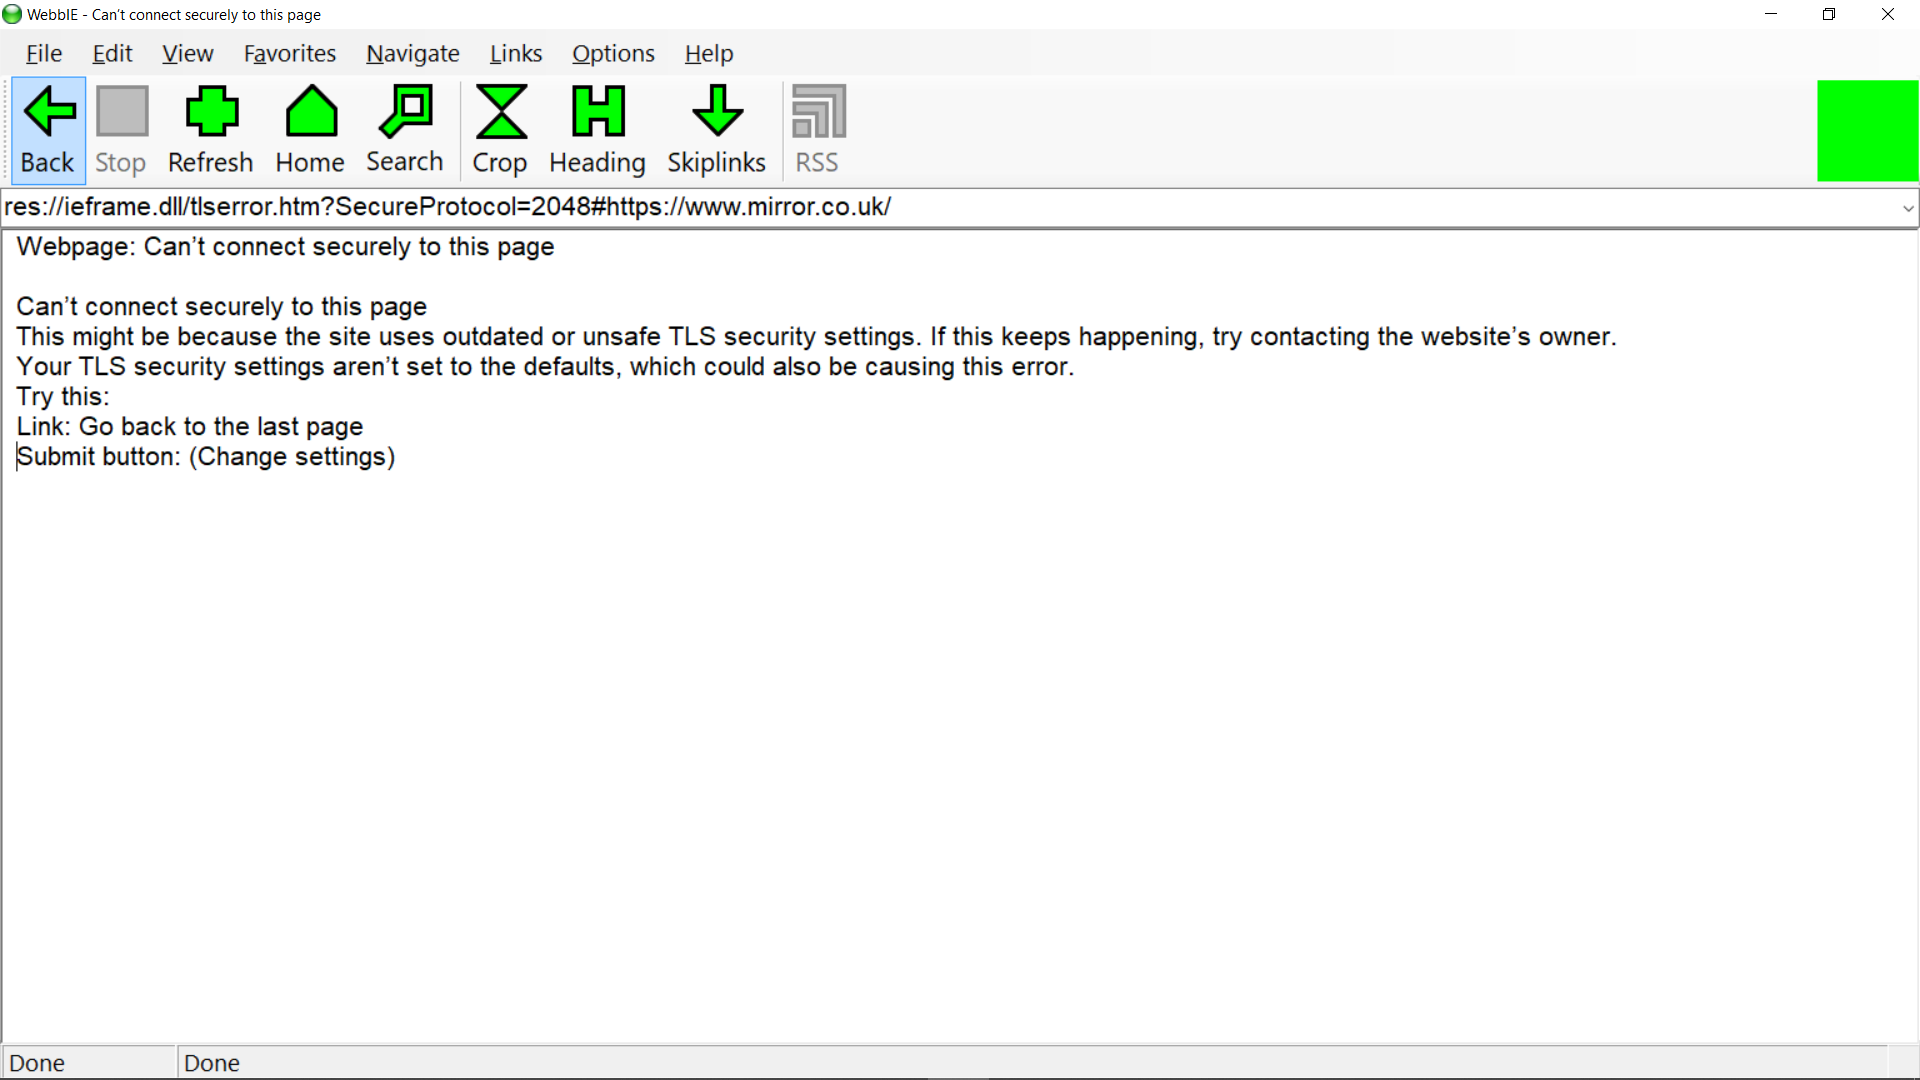
\includegraphics[keepaspectratio,width=\linewidth]
        {images/webbie-mirror}
        
        \caption[WebbIE browser]
        {%
        Browsing the mirror.co.uk website
        }
        \label{fig:webbie-mirror}
    \end{minipage}
\end{figure}

\subsection{Basic Data About Text-Only Browsers}
\begin{table}[tp]
    \tablestretch
    \rowcolors{2}{}{tablerowcolour}
    \centering
    \begin{tabularx}{\linewidth}
    {>{\kern-\tabcolsep}llXX<{\kern-\tabcolsep}}
    \toprule
    \textbf{Browser} & \textbf{Last update} & \textbf{System} & \textbf{Licence} \\
    \midrule
    Lynx & 2020, Feb, 27 (v2.9.0) & Linux & Free \\
    %
    WebbIE & 2021, Dec, 23 (v5.1.0) & Windows & Free \\
    %
    W3M & 2022, Sep, 17 (v2.28) & Linux & Free \\
    %
    Links & 2022, Sep, 17 (v2.28) & Linux & Free \\
    %
    \bottomrule
    \end{tabularx}
    
    \caption[Text-Only Browser Information]
    {
    Information of text browsers
    }
    \label{tab:text-browsers-info}
\end{table}